%% ----------------------------------------------------------------
%% Thesis.tex -- MAIN FILE (the one that you compile with LaTeX)
%% ---------------------------------------------------------------- 

% Set up the document
\documentclass[a4paper, 12pt, oneside]{Thesis}  % Use the "Thesis" style, based on the ECS Thesis style by Steve Gunn
\graphicspath{Figures/}  % Location of the graphics files (set up for graphics to be in PDF format)

% Include any extra LaTeX packages required

\usepackage{titlesec}
%\usepackage{float}
\usepackage{pbox}
\usepackage[square, numbers, comma, sort&compress]{natbib}  % Use the "Natbib" style for the references in the Bibliography
\usepackage{verbatim}  % Needed for the "comment" environment to make LaTeX comments
%\usepackage{graphicx}
\usepackage{caption} \captionsetup[table]{skip=0pt}
%\usepackage{subcaption}
\usepackage{subfigure}
\usepackage{setspace}
\usepackage{vector}  % Allows "\bvec{}" and "\buvec{}" for "blackboard" style bold vectors in maths
\usepackage{amsmath}
\hypersetup{urlcolor=black, colorlinks=true}  % Colours hyperlinks in blue, but this can be distracting if there are many links.
%\usepackage{nomencl}
%\makeglossary
\usepackage{floatrow}
%\usepackage[demo]{graphicx}
\usepackage{multicol}
%\usepackage{minipage}
\usepackage{courier}
\usepackage{amsmath}
\usepackage{amssymb}
\usepackage{graphicx}
\usepackage{caption}
%\usepackage{subcaption}
%\usepackage{float}
\usepackage{bm}
\usepackage[hypcap]{caption}
\usepackage{multirow}
\usepackage{soul}
\usepackage{pifont} 
\usepackage{booktabs}
\usepackage{lineno}
\usepackage{program}
\usepackage{algorithmic}
\usepackage{setspace}
\usepackage{color}
\usepackage{booktabs}
\usepackage{longtable}
\usepackage{pdflscape}

%% ----------------------------------------------------------------
\begin{document}
	\frontmatter      % Begin Roman style (i, ii, iii, iv...) page numbering
	\setstretch{1.5} 
	\thispagestyle{empty}
	\newpage
	\null
	\setcounter{page}{0}
	\parskip=0pt
	\begin{center}%
		
		\let \footnote \thanks
		\vglue 0in % this makes top margin 2in
		%\vskip 5ex%
		\begin{spacing}{1.6}
			\textbf{\Large  LINUX BASED TELECOMMAND DATA SYSTEM DEVELOPMENT PROJECT}
		\end{spacing}
		\vspace{12 mm}
		{\bf \em SOFTWARE DESIGN (SDD)
			DOCUMENT \newline version 2.0
		}\par
		\vskip 6ex%
		
		\vspace*{0.25in}
		\begin{figure}[H]
			\begin{tabular}{ccc}
				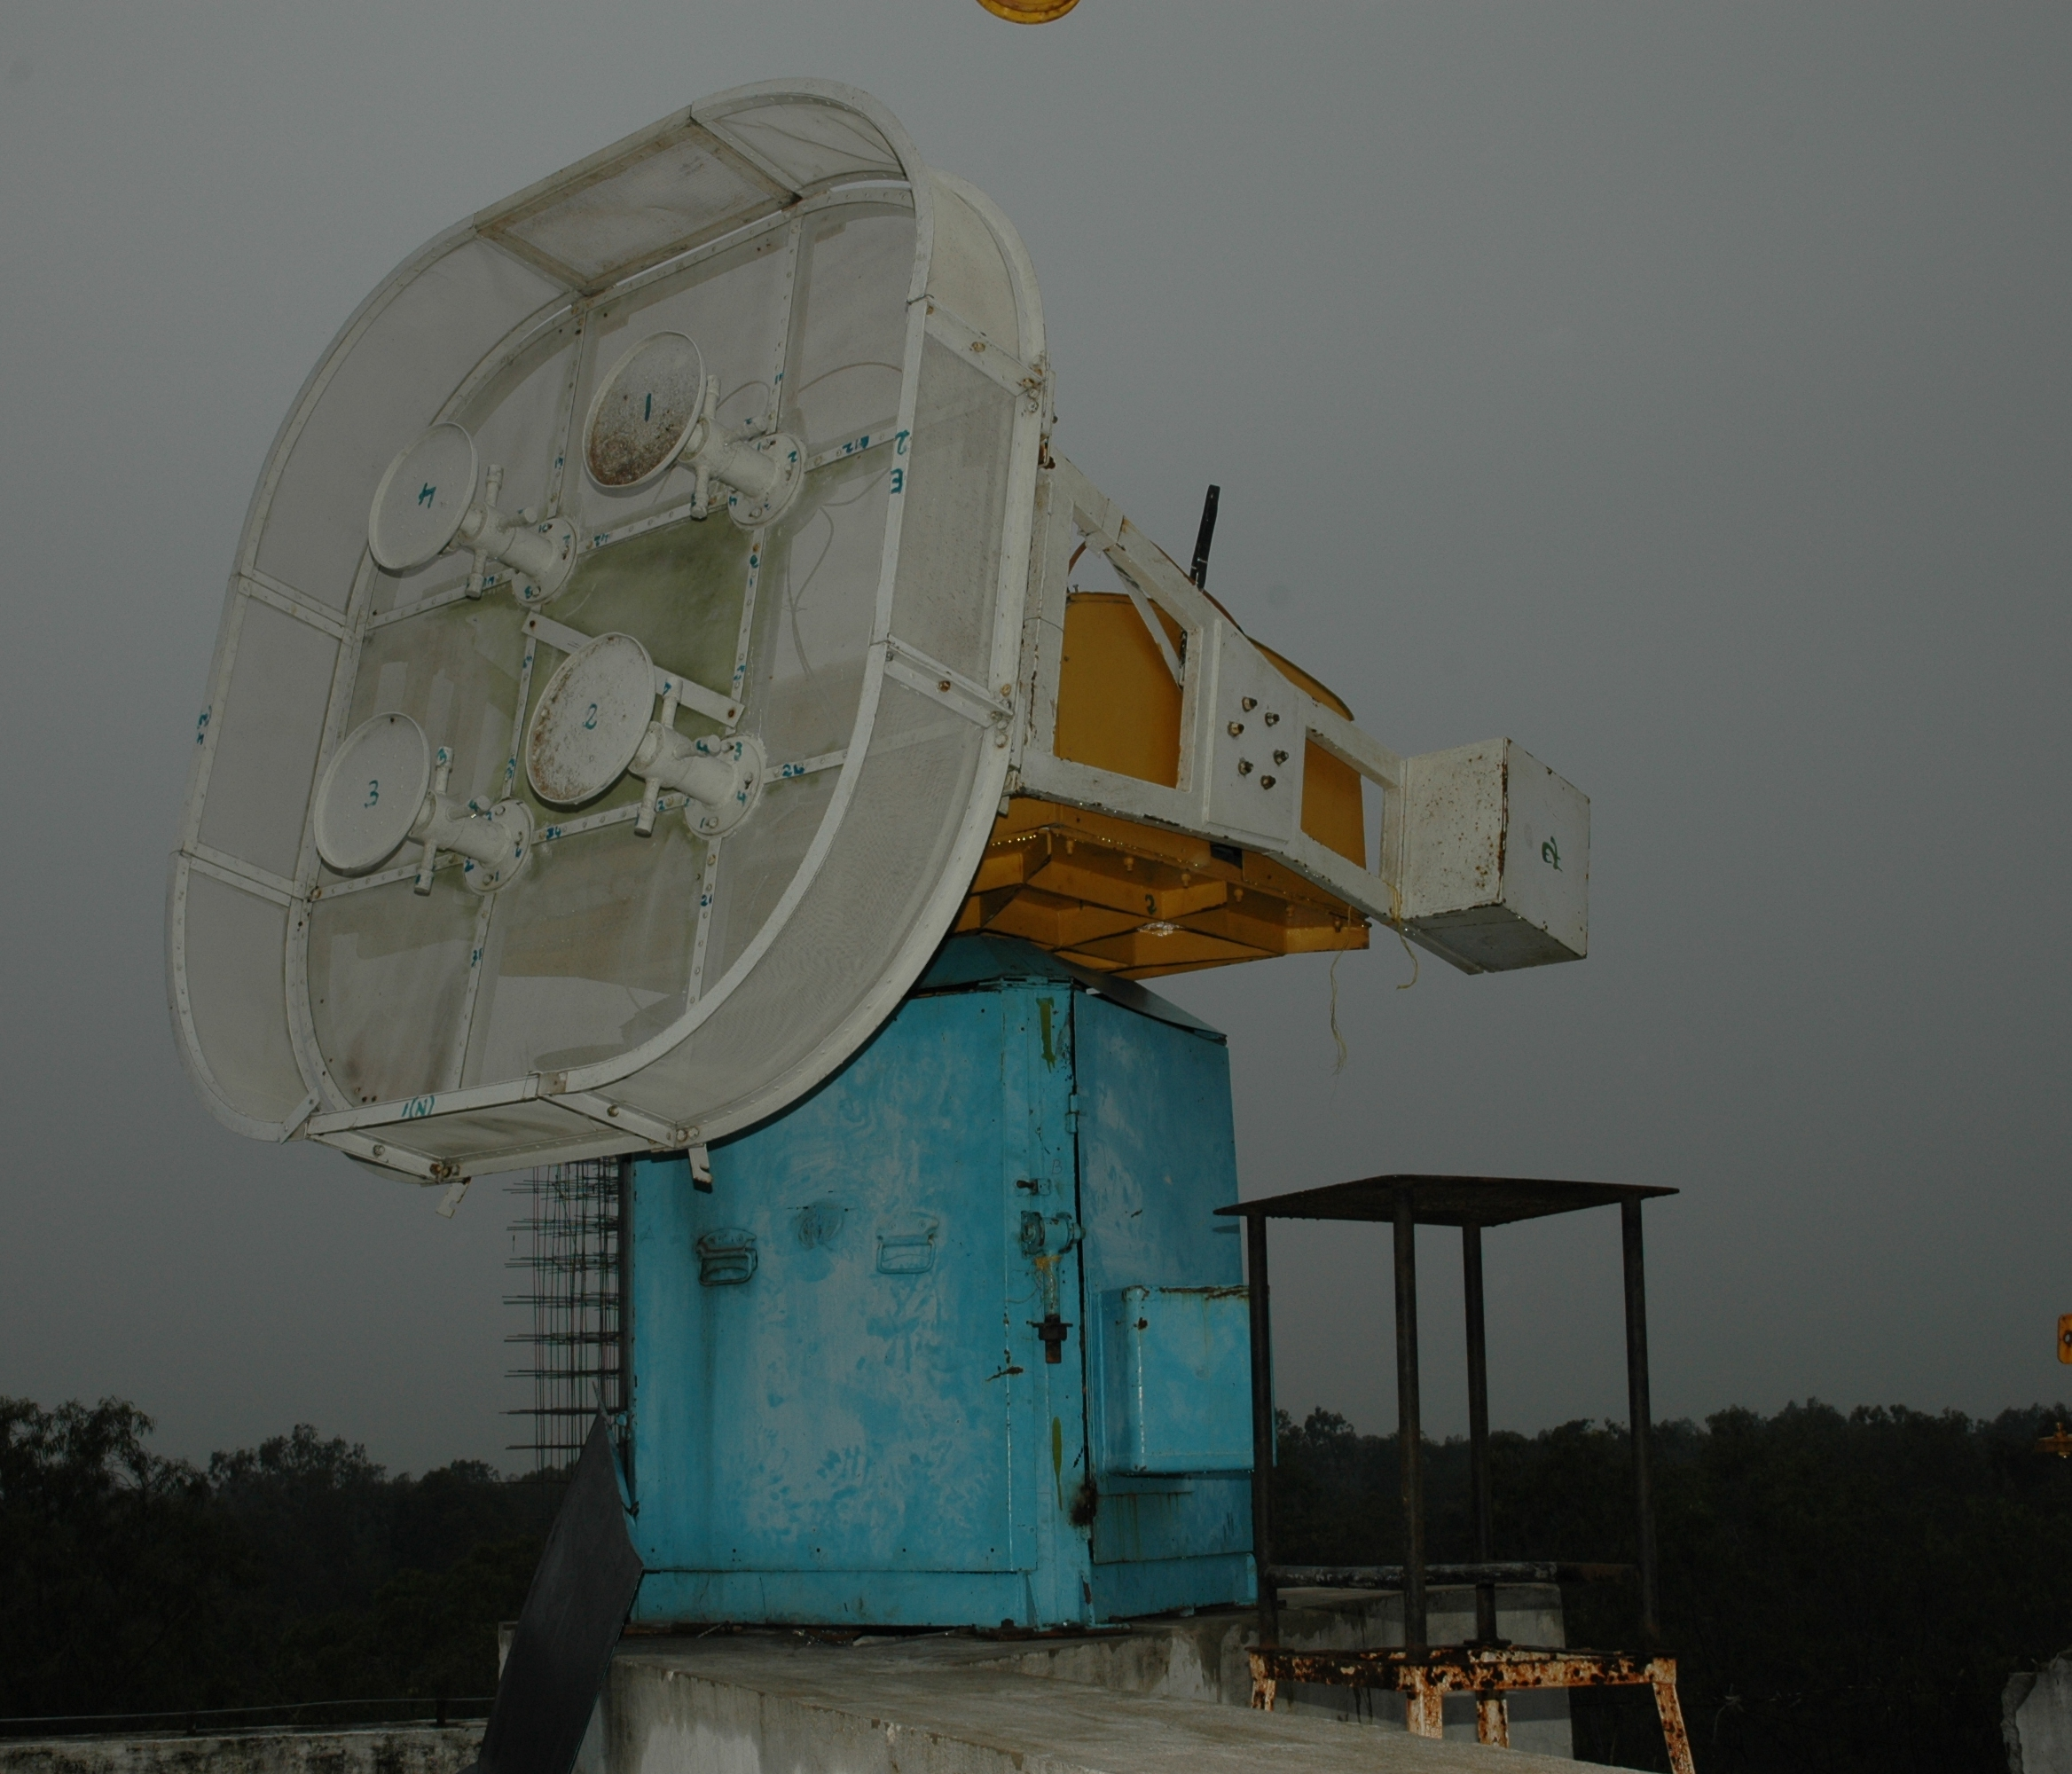
\includegraphics[height=1.5in, width=1.65in]{./AntElement.jpg}&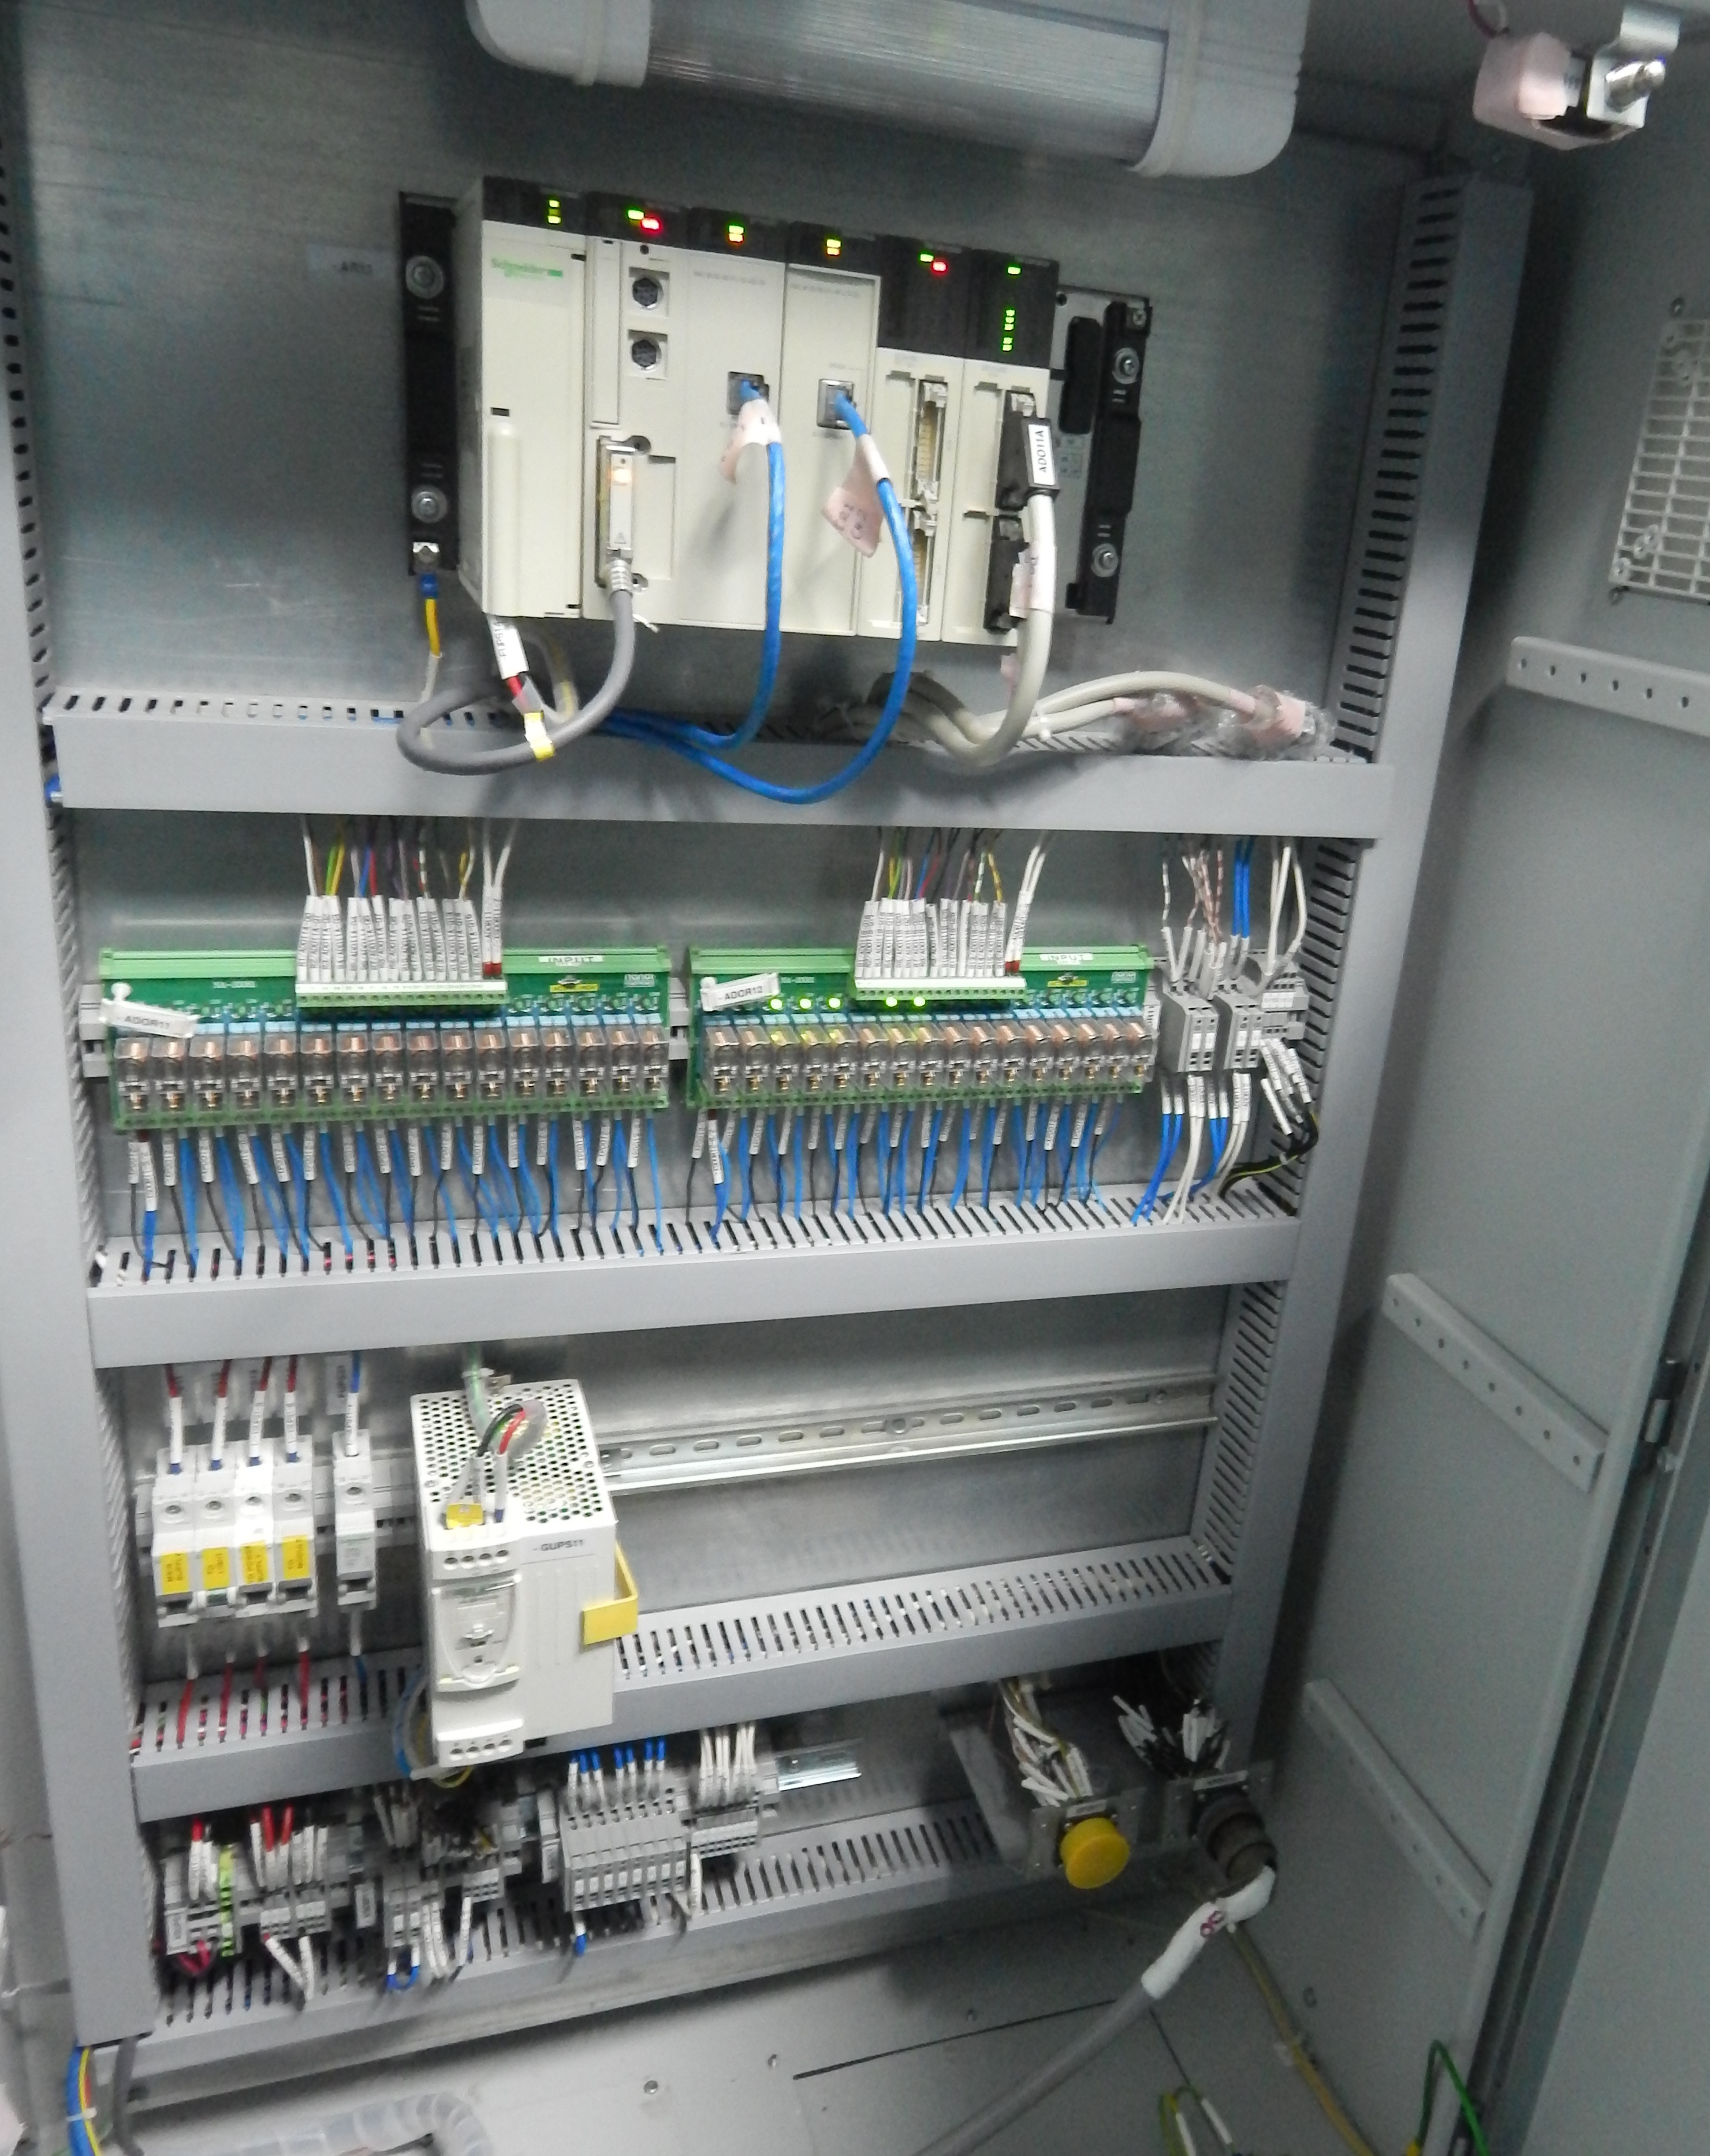
\includegraphics[height=1.5in,width=1.65in]{./CRI1.jpg}&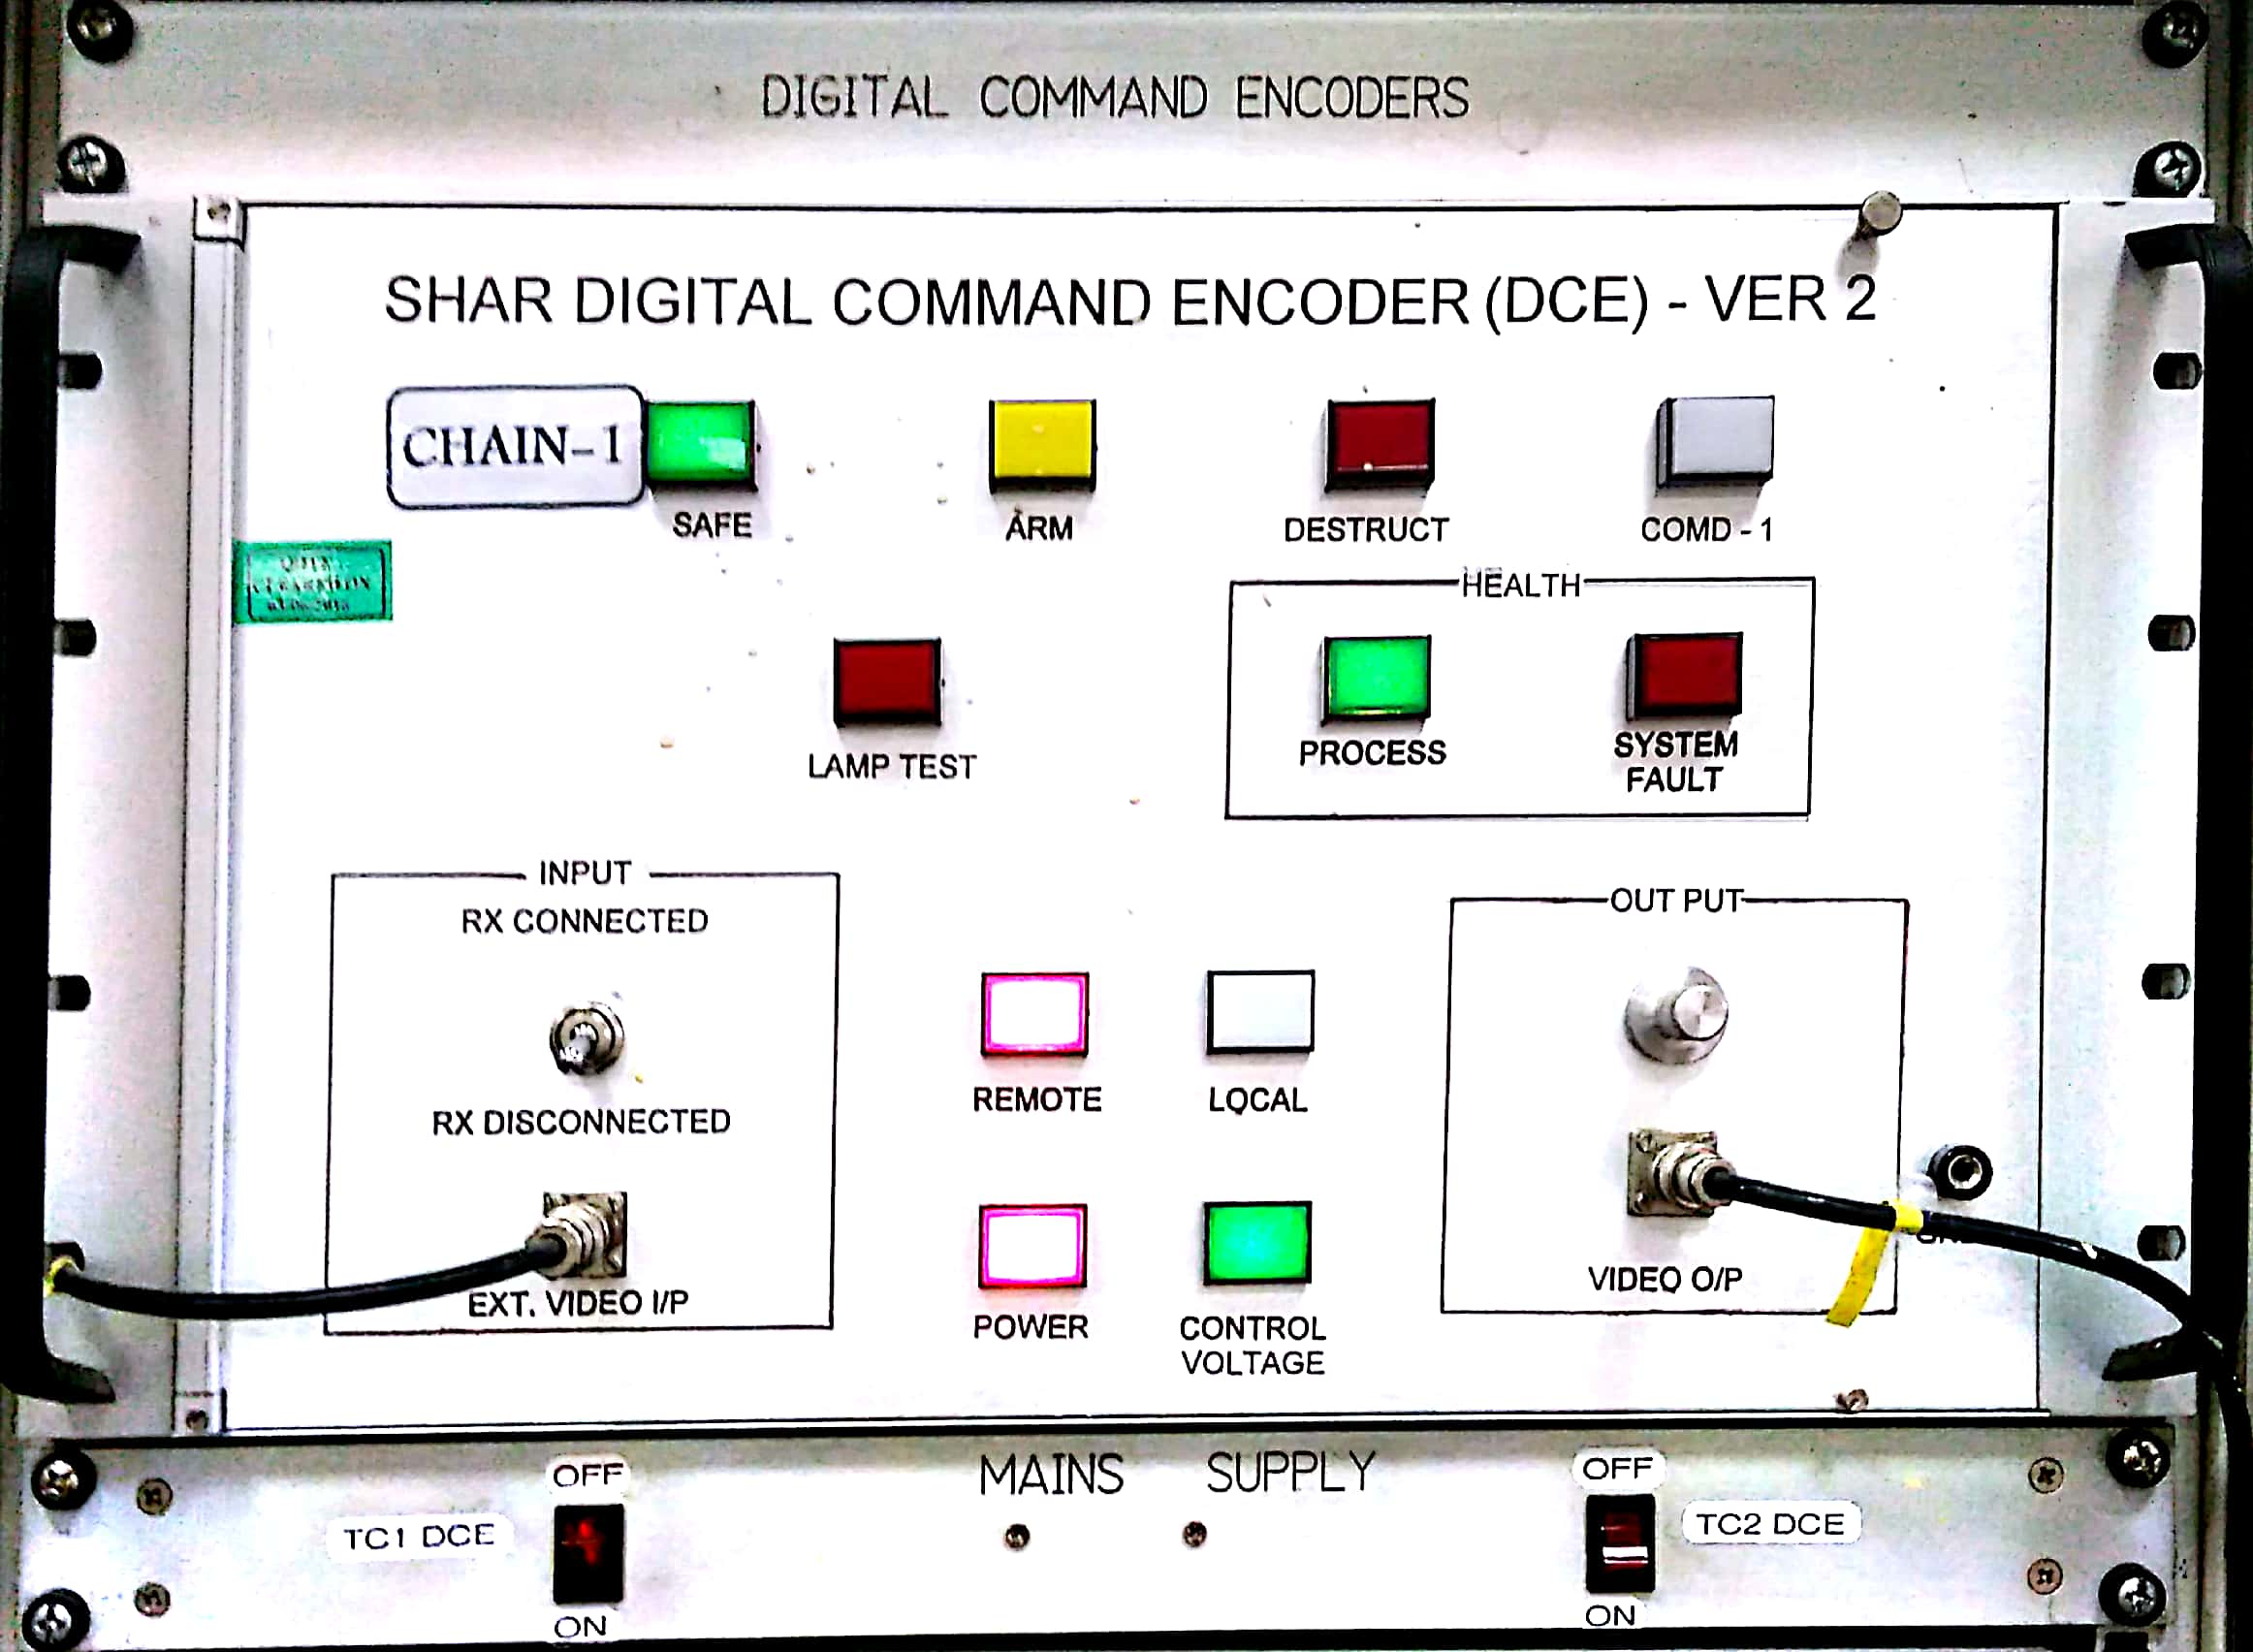
\includegraphics[height=1.5in,width=1.65in]{./DCE.jpg}\\
				
				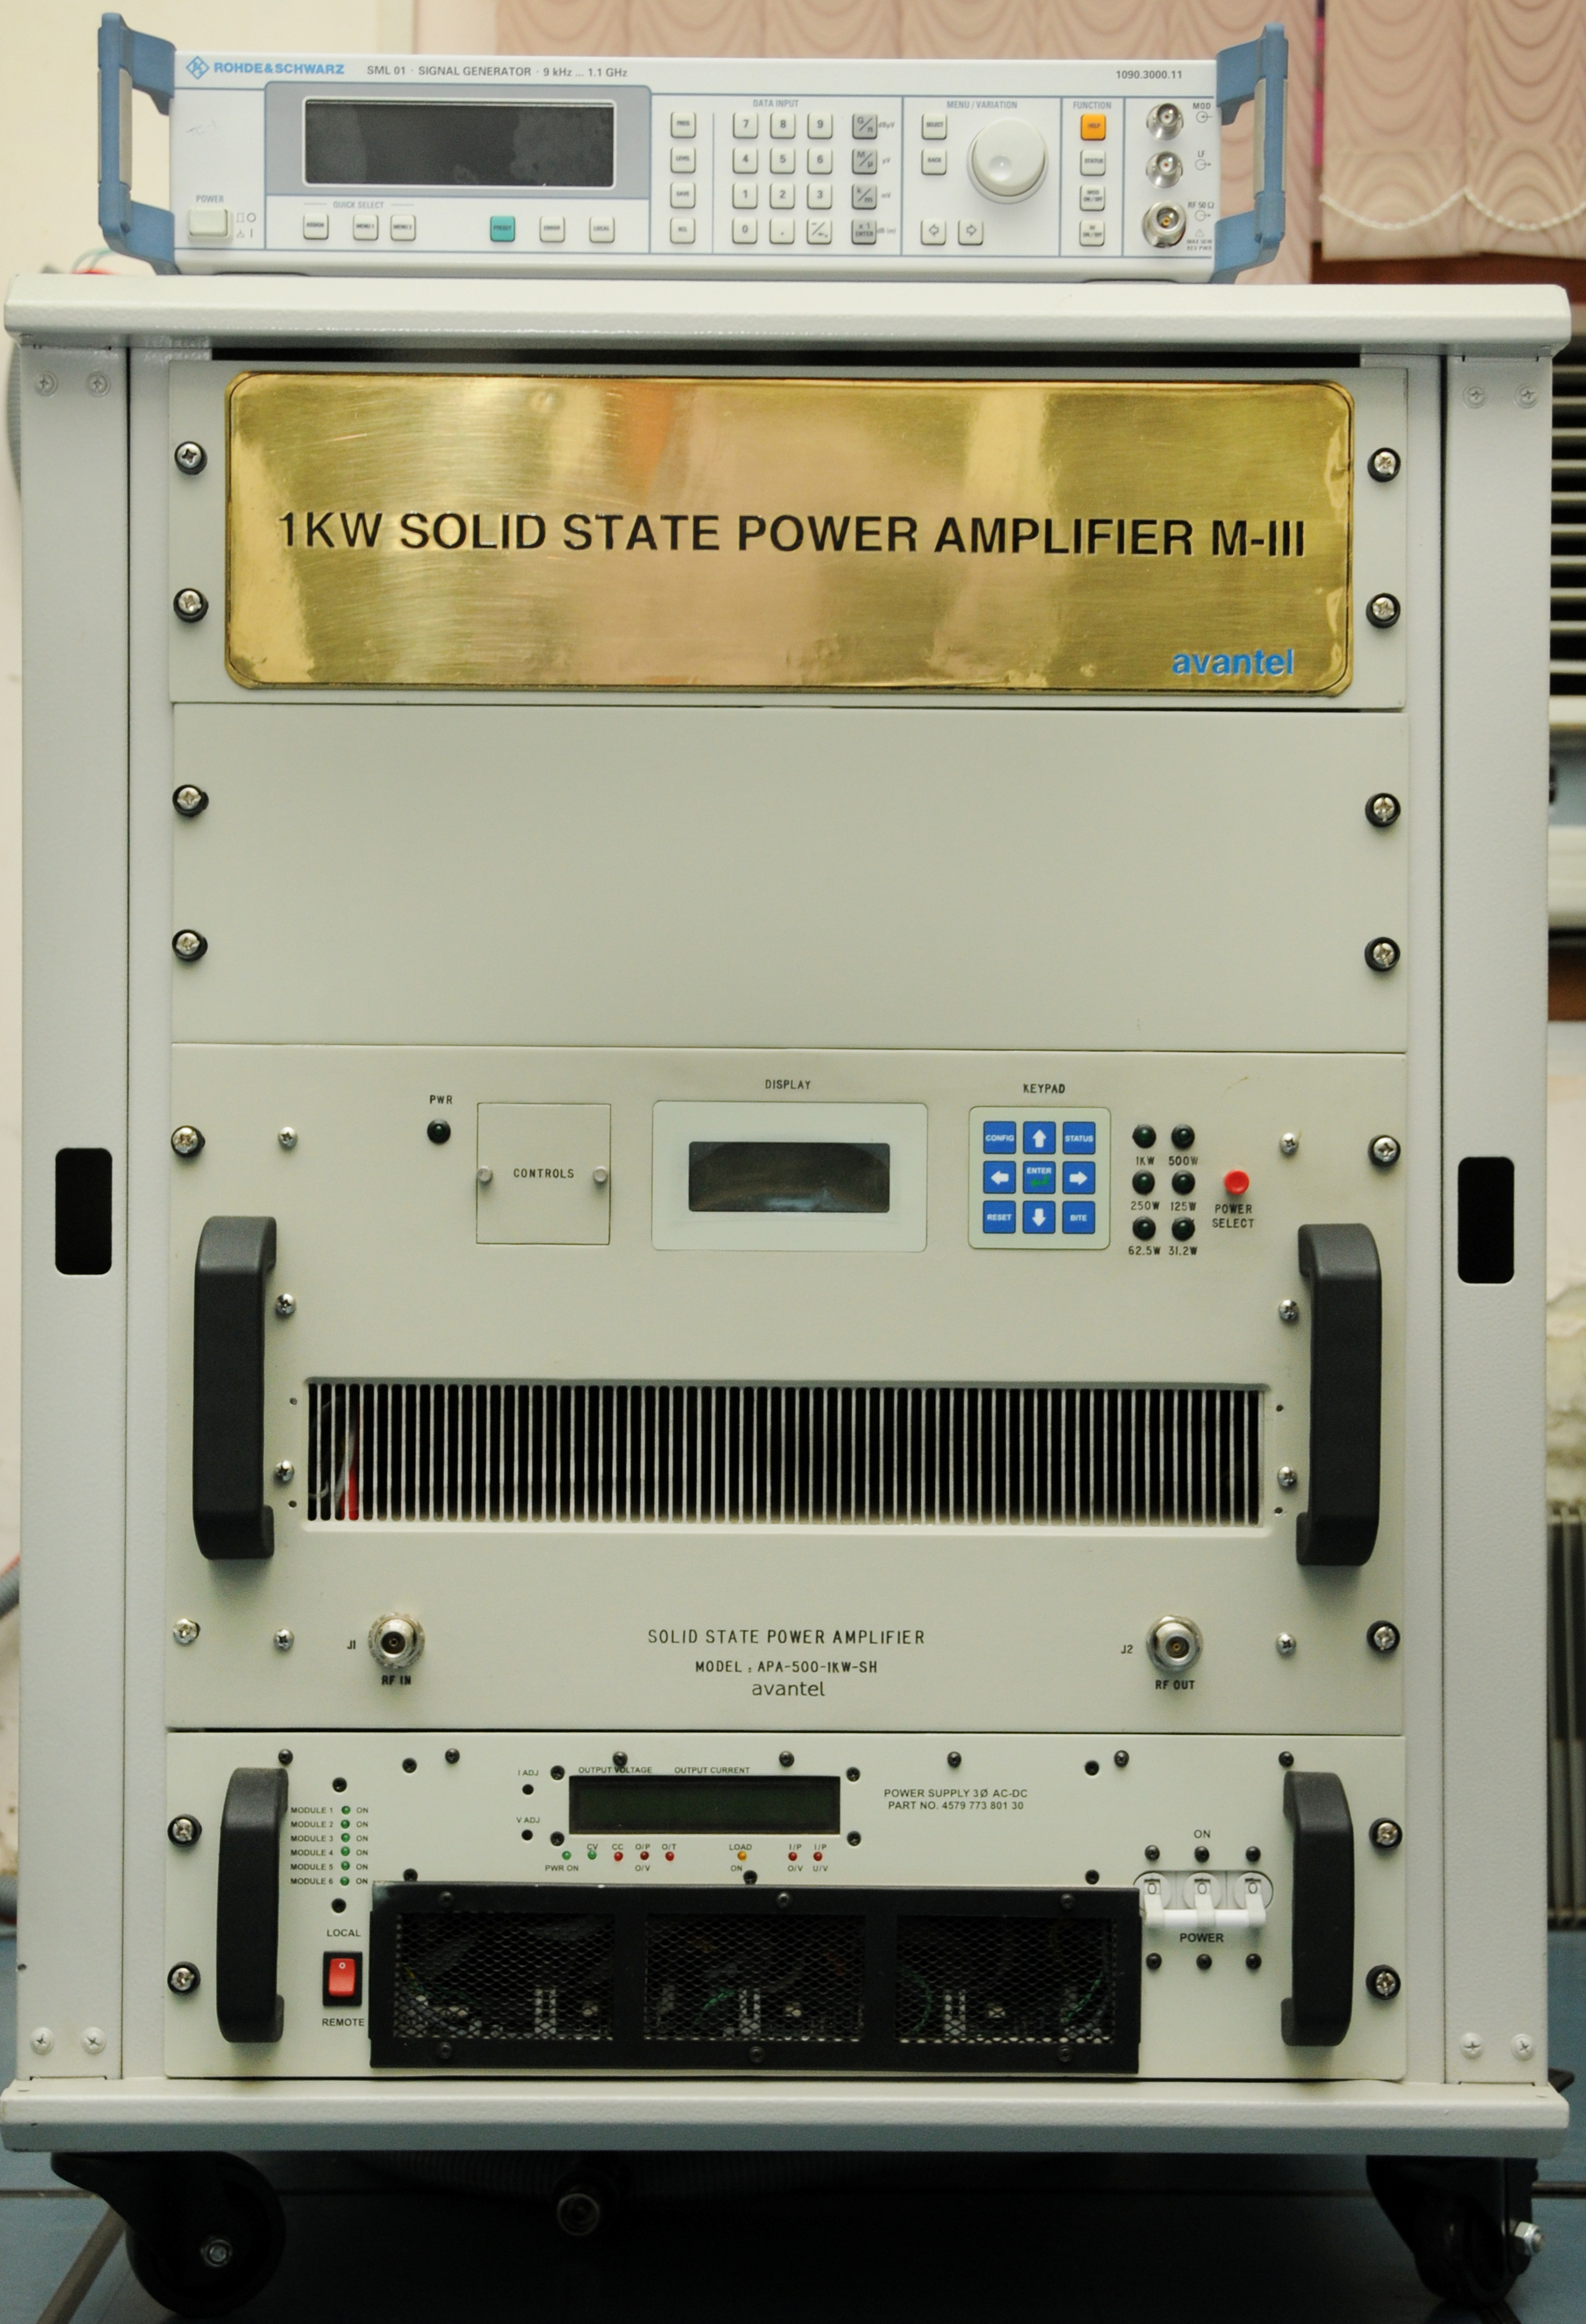
\includegraphics[height=1.5in,width=1.65in] {./NewPA.jpg}&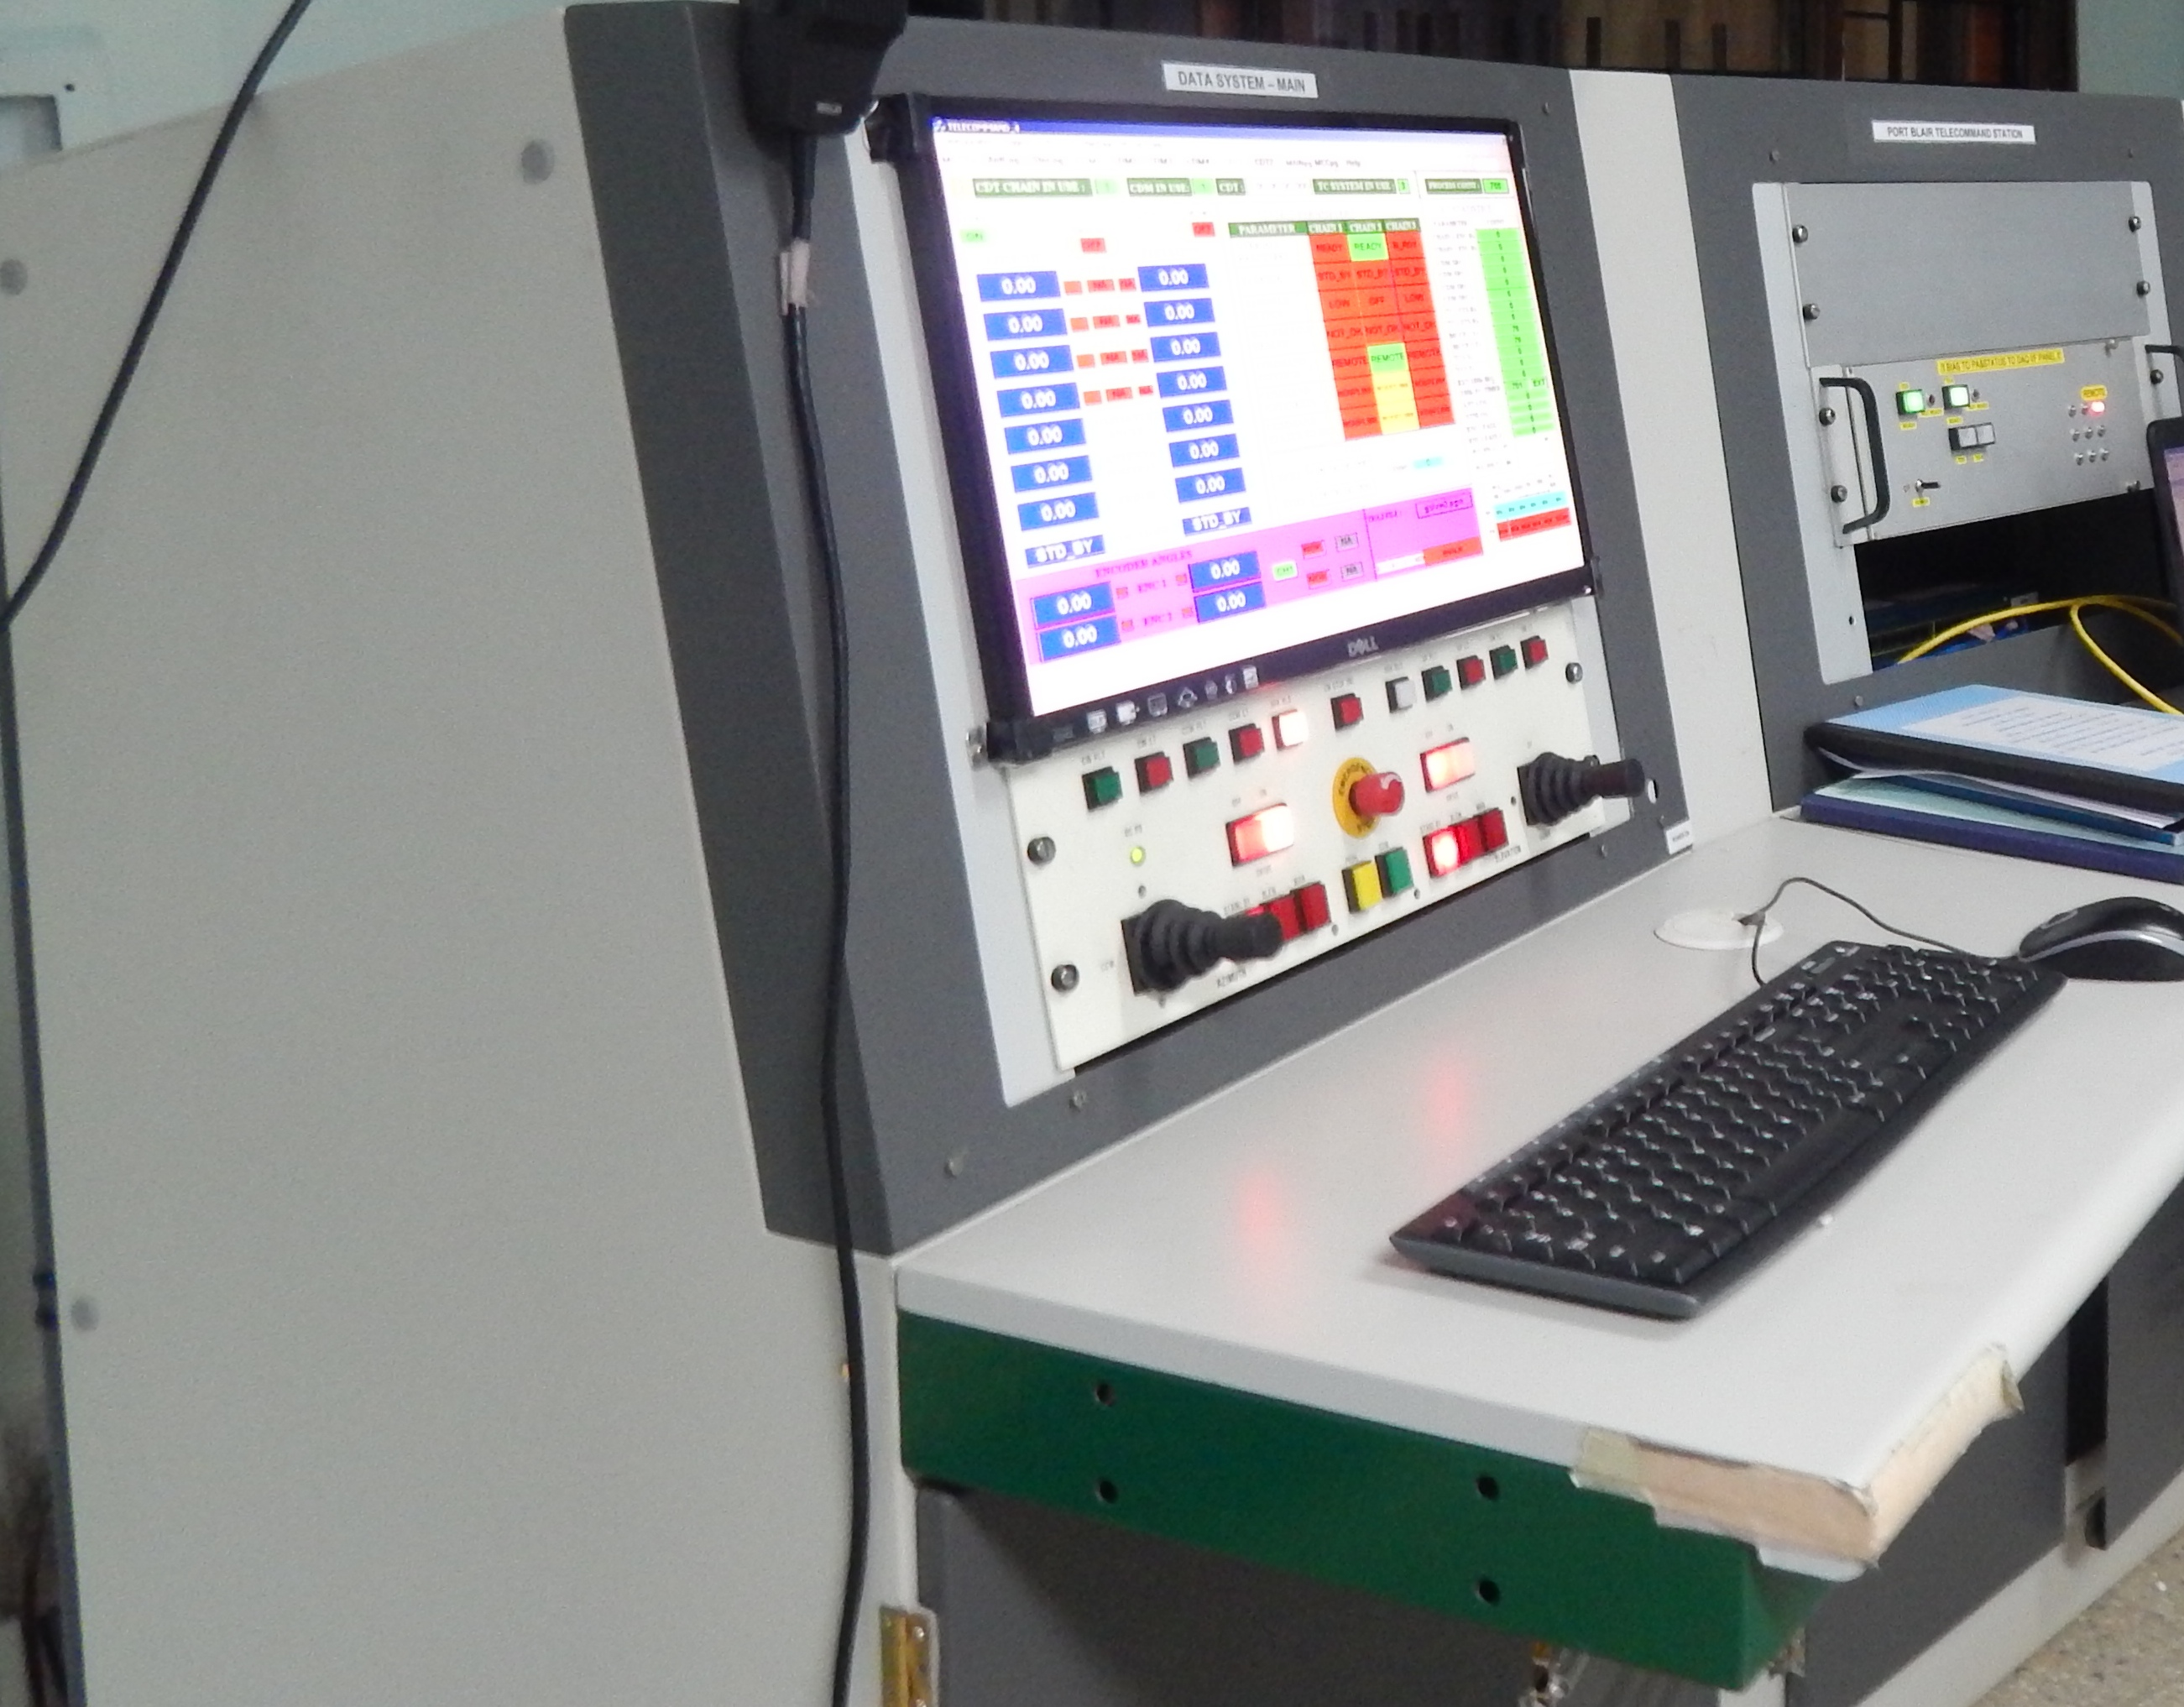
\includegraphics[height=1.5in,width=1.65in]{./Console1.jpg}&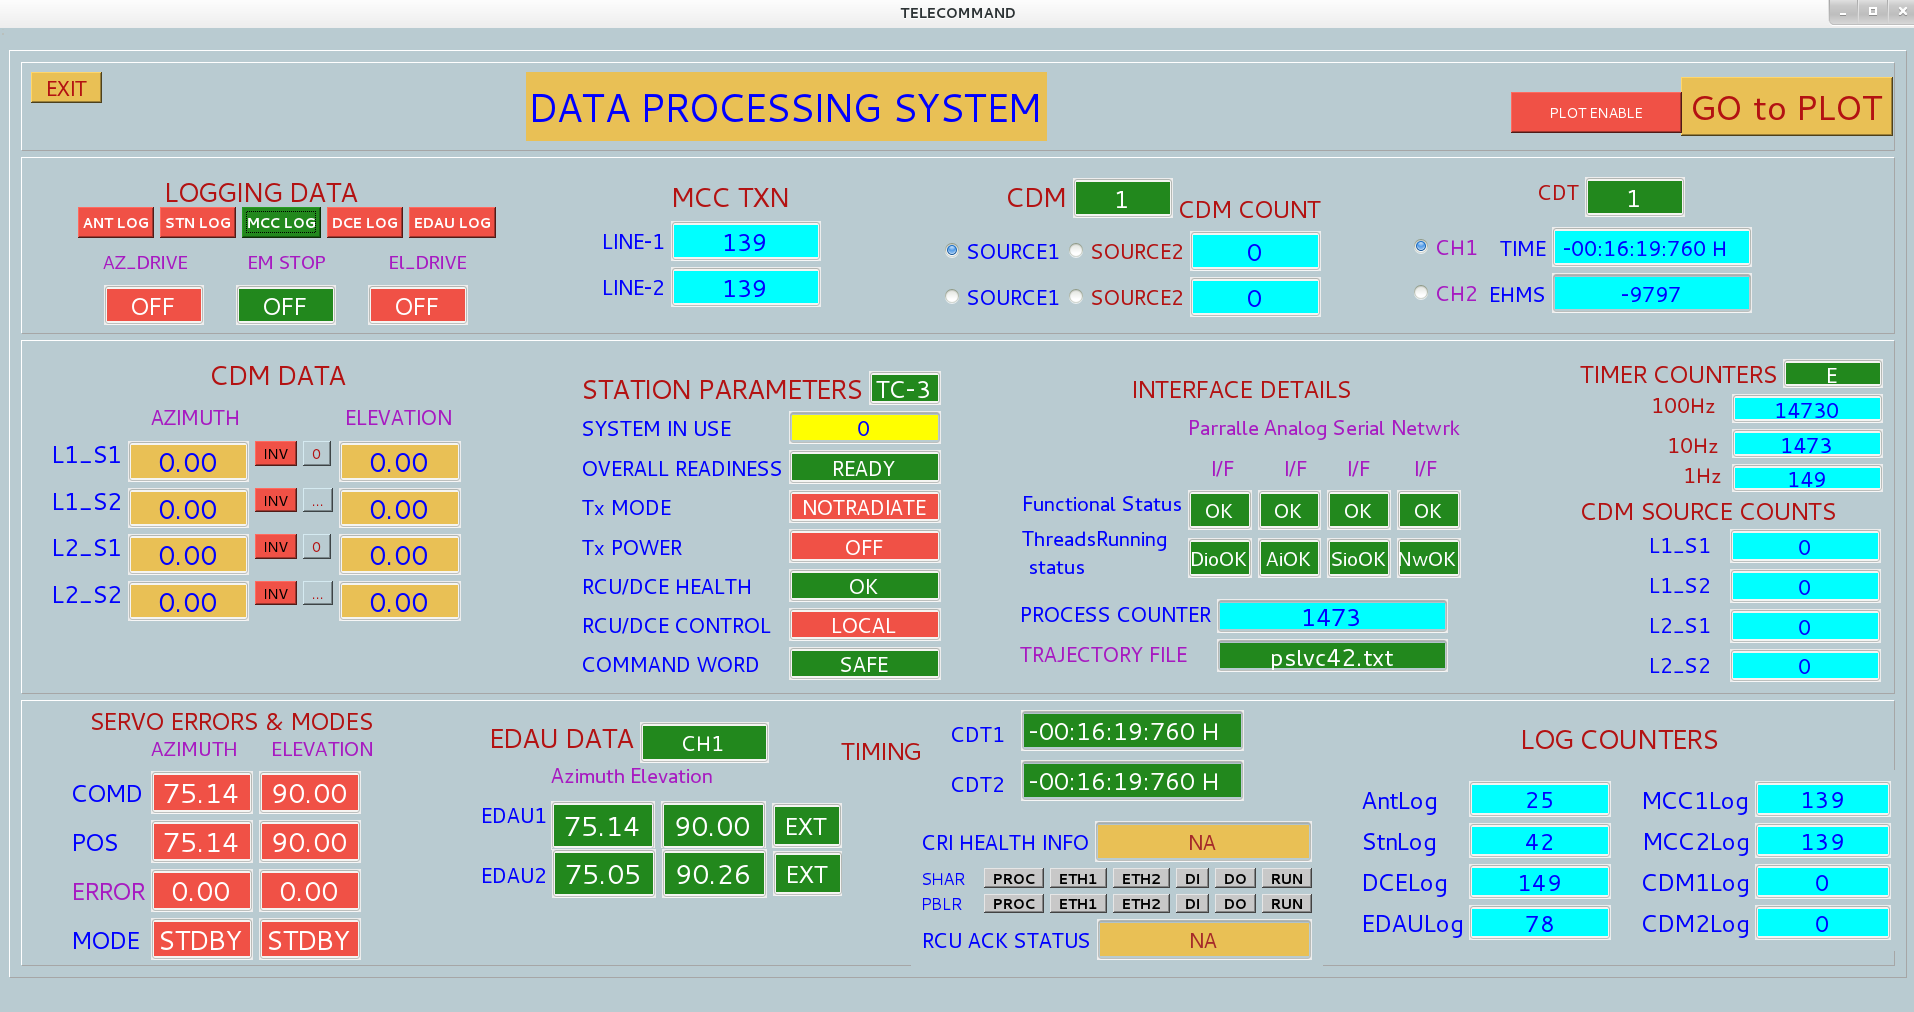
\includegraphics[height=1.5in,width=1.65in]{./MainPage.png}\\
				
			\end{tabular}
			
		\end{figure}
		
		\vspace*{0.25in}
		
	\end{center} 
	\begin{center}
		{\bf \large \MakeUppercase{ TELECOMMAND}\par} 
		{\hspace*{0.4in} \bf RANGE INSTRUMENTATION SYSTEMS \newline RANGE OPERATIONS\\
			SATISH DHAWAN SPACE CENTER}
		\vglue 0.50em
		{\bf \large August 2018\par }%\@date}\par
	\end{center}
	%\parskip 8pt
	
	
	
	
	%%%%%%%%%%%%%%%%%%%%%%%%%%%%%%%%%%%%%%%%%%%%%%%%%%%%%%%%%%%%%%%%%%%%%%
	%\newpage
	%\input{certificate}
	\newpage
	\vspace*{36pt}
	\begin{center}
		
		
		\let \footnote \thanks
		\vglue 0in % this makes top margin 2in
		%\vskip 5ex%
		\begin{spacing}{1}
			\textbf{\Large  LINUX BASED TELECOMMAND DATA SYSTEM DEVELOPMENT PROJECT}
		\end{spacing}
		
	\end{center}  
	%\vskip 25pt
	%\thispagestyle{empty}
	
	%\setcounter{page}{0}
	\pagenumbering{roman}
	
	
	\noindent 
	
	
	
	
	\vspace*{1in}
	
	\parbox{1.8in}
	{
		\noindent {\bf Prepared By} \\
		\noindent {\bf } \\
		\noindent             M ASHOK KUMAR \\ 
		\noindent Engineer-SC\\
		\noindent TC/RIS/RO\\
	} 
	\hspace*{0.20in} 
	\parbox{1.5in}
	{
		\noindent {\bf} \\
		
		\noindent             K HARIBABU\\ 
		\noindent Engineer-SE\\
		\noindent TC/RIS/RO\\
		
		
	}  
	\hspace*{0.20in} 
	\parbox{1.8in}
	{
		\noindent {\bf} \\
		
		\noindent             P VIJAYALAKSHMI\\ 
		\noindent Engineer-SE\\
		\noindent TC/RIS/RO\\
		
		
	}
	
	\vspace*{0.25in}
	
	\parbox{2.2in}
	{
		\noindent {\bf} \\ \\
		\noindent {\bf Checked $\&$ Verified By} \\
		\noindent {\bf} \\
		\noindent             K RAJENDRABABU \\ 
		\noindent Manager\\
		\noindent TC/RIS/RO\\
		\noindent {\bf} \\
		\noindent {\bf} \\
	} 
	\parbox{2.2in}
	{
	\noindent {\bf } \\
	\noindent {\bf } \\
	\noindent J GOPALAKRISHNA \\ 
	\noindent General Manager\\
	\noindent RIS/RO\\
	} 
\hspace*{0.20in} 
	
	\vspace*{0.25in}
	
	\parbox{2.2in}
	{
		\noindent {\bf Reviewed \& Approved By} \\
		\noindent {\bf} \\
		\noindent             V SESHAGIRI RAO \\ 
		\noindent Chairman\\
		\noindent STARS\\
	} 
	\newline
	\hspace*{2.5in}
	\noindent Sriharikota\\
	\hspace*{2.4in}
	August, 2018
	\clearpage
	%%---------------------------------------------\clearpage
	\vspace*{36pt}
	%\declaration
	\begin{center}
		{\large \bf CERTIFICATE}
	\end{center}
	
	
	\vspace*{24pt}
	
	% Please add the following required packages to your document preamble:
	% \usepackage{booktabs}
	\begin{table}[h]
		\centering
		%	\caption{Certificate}
		\label{TAB:Certificate}
		\begin{tabular}{@{}lll@{}}
			\toprule
			\textbf{Sl No} & \textbf{Parameter}           & \textbf{Description}                           \\ \midrule
			1              & Security                     & \textbf{Restricted}                            \\
			2              & Status                       & \textbf{Revised}                                   \\
			3              & Document No                  & ISRO-SHAR-03-R-TR-168-2017                              \\
			4              & Type of Document             & TR - Technical Report                          \\
			5              & Title \& Sub-title           & Software Design Document for \\
			&                              & Linux Based Telecommand Data Systems           \\
			6              & Author(s)                    & M Ashok Kumar, Engineer-SC, TC/RIS/RO \newline    \\
			&                              & K Haribabu, Engineer-SE, TC/RIS/RO           \\
			&                              & P Vijayalakshmi, Engineer-SE, TC/RIS/RO           \\
			7              & Checked $\&$ Verified   & K Rajendrababu, Manager, TC/RIS/RO           \\                  
			& & J Gopalakrishna, General Manager, RIS/RO      \\
			8              & Reviewed                     & STARS                                          \\
			9              & Approved                     & STARS                                          \\
			10             & Originating Agency           & Satish Dhawan Space Center, SDSC SHAR          \\
			11             & Month \& Year of Publication & August, 2018                                  \\
			12             & No. of Pages                 & 16+186                                             \\
			13             & No. of Figures               & 12                                             \\
			14             & No. of Tables                & 09                                             \\
			15             & No. of References            & 06                                             \\
			16             & No. of Enclosures            & Verification\&Validation, Test\&Evaluation document                                            \\ \bottomrule
		\end{tabular}
		
		
	\end{table}
	
	\parbox{2.9in}{
		
	}  
	
\clearpage
%%---------------------------------------------
\clearpage
\vspace*{36pt}
%\declaration
\begin{center}
{\large \bf CHANGE HISTORY}
\end{center}


\vspace*{24pt}

% Please add the following required packages to your document preamble:
% \usepackage{booktabs}
\begin{table}[h]
	\centering
	%	\caption{Certificate}
	\label{TAB:Certificate}
	\begin{tabular}{@{}lll@{}}
		\toprule
		\textbf{Sl No} & \textbf{Parameter}           & \textbf{Description}                           \\ \midrule
		1              & Project Name           & Software Design Document (SDD) for \\
		&                              & Linux Based Telecommand Data Systems           \\
		2              & Plan Version No                      & 2.0      \\
		3              & Date of release                   & 29-08-2018                                          \\
		4              & Approved by                     & STARS                                          \\
		             & Signature          &           \\
		5            & No. of pages &  NA                                 \\
		6             & List of pages for changes made                 &   NA                                         \\
		7             & List of previous version Nos      &  NA                                            \\
		8             & Dates of release of previous versions     &  NA                \\
		 \bottomrule
	\end{tabular}
	
	
\end{table}
\parbox{2.9in}

\vspace*{0.25in}

%%%%%%%%%%%%%%%%%%%%%%%%%%%%%%%%%%%%%%%%%%%%%%%%%%%%%%%%%%%%%%%%%%%%%



\setstretch{1.3}  % It is better to have smaller font and larger line spacing than the other way round

% Define the page headers using the FancyHdr package and set up for one-sided printing
\fancyhead{}  % Clears all page headers and footers
\rhead{\thepage}  % Sets the right side header to show the page number
\lhead{}  % Clears the left side page header

\pagestyle{fancy}  % Finally, use the "fancy" page style to implement the FancyHdr headers

%% ----------------------------------------------------------------

%%%%%%%%%%%%%%%%%%%%%%%%%%%%%%%%%%%%%%%%%%%%%%%%%%%%%%%%%%%%%%%%%%%% ----------------------------------------------------------------
\clearpage  % Declaration ended, now start a new page
% The Abstract Page
\setstretch{1.4}


%\abstract{

\addtocontents{toc}{\vspace{0em}}
\begin{center}
\LARGE\textit{Abstract}
\end{center}
\vspace{-3 mm}
\begin{spacing}{1.3}

Development of Linux based Data Systems for Telecommand is being carried out with in-house design. This document describes the Software Requirements Specifications (SRS) for Linux based Telecommand Data System Development. The base line reference for the preparation of this document are exisiting windows based software design document \cite{TCOldSWDoc}, station manual of Telecommand \cite{TCOldStnMan}, CRI software design document \cite{CRISWDoc}, CRI software requirements specifications \cite{CRISRS}, Linux DPS systems requirement document \cite{SYRSLBDPS}, and Linux DPS software requirements document \cite{SRSLBDPS}. \\

Data Processing System going to be housed in Telecommand at SHAR and Portblair does the following for range safety purpose (i) used to drive the Telecommand antenna by means of servo control system to point towards the launch vehicle during real time, (ii) RSO command status acquisition, (iii) radiated power level of Power Amplifier, status of Servo system, Radiation chain control, Timing information acquisition, antenna pointing information, encoder auto change over based on health parameters, (iv) servo error generation, (v) CDM reception, (vi) MCC transmission, (vii) acquisition, framing, processing and pecketisation of data and (viii) logging to hard disk at different rates.\\

This document is made as per the guidelines of the ISPD and follows the IEEE STD 1233-1998. The document is organized as 10 sections. Section \ref{Chapter1} describes purpose of the system and its sub-systems. It also presents the scope and over view of the entire system. In section \ref{Chapter2}, decomposition descripton is given. This includes module level decomposition, concurrent process decomposition and data decomposition. Dependency description which includes intermodule dependency, interprocess dependency and data dependencies, is provided in section \ref{Chapter3}. Interface description  of module and process are given in section \ref{Chapter4}. Detailed design containing modules detailed design, threads detailed design, data detailed design are explained in section \ref{Chapter5}. Section \ref{Chapter6} gives the procedures for loading OS and add on drivers along with useful commands. Details of various data logging formats, interconnections, configuration files and pin assignments are presented in section \ref{Chapter7}. Flow charts are given in section \ref{Chapter8} which details the flow of code. Section \ref{Chapter9} presents the features of new linux based Data Systems compares to that of old windows 2K based Data Systems. Finally, section \ref{Chapter10} provides the GUI pages  of linux Data System with description.



\end{spacing}

\clearpage  % Abstract ended, start a new page
%% ----------------------------------------------------------------
\setstretch{1.4}


%\abstract{

\addtocontents{toc}{\vspace{0em}}
\begin{center}
\LARGE\textit{Keywords}
\end{center}
\vspace{10 mm}
\begin{spacing}{1.5}


%Probabilistic Models \\
%Boltzmann Machines \\
Graphical User Interface\\
Absolute Rotary Encoder\\
Linux Operating System\\ 
Serial Communication\\
Digital Command Encoder Unit\\  
Amplifier Bias\\
Control Panel\\
Range Safety\\
Receiver\\
Antenna\\
Driver Amplifier\\
Demodulator\\
Convolutional Encoder\\
Viterbi Decoder\\
\end{spacing}

\clearpage  % keywords Ended here
%% ----------------------------------------------------------------


%\addtocontents{toc}{\vspace{0em}}
%\begin{center}
%\LARGE\textit{Acronyms}
%\end{center}
%\vspace{10 mm}
%\begin{spacing}{1.5}
%CNN\:			: Convolutional Neural Network\\
%DL\:			: Deep Learning\\
%RBM\:			: Restricted Boltzman Machine\\
%FBP\:			: Feed Back Propagation\\
%WM\:			: WaterMark\\
%CB\:			: Code Book\\
%DCT\:			: Discrete Cosine Transform\\
%DWT\:			: Discrete Wavelet Transform\\
%SVD\:			: Singular Value Decomposition\\
%SWT\:			: Stationery Wavelet Transform\\
%
%
%			
%\end{spacing}
%
%\clearpage  % Acronyms Ended here
 ----------------------------------------------------------------

\setstretch{1.5}  % Reset the line-spacing to 1.3 for body text (if it has changed)

% The Acknowledgements page, for thanking everyone

\acknowledgements{
\addtocontents{toc}{\vspace{1em}}  % Add a gap in the Contents, for aesthetics
 
\paragraph*{}  
%We express our sincere gratitude to Dr. Sai Subrahmanyam Gorthi, Associate Professor, IIST and Dr Deepak Mishra, Associate Professor, IIST for their guidance, enthusiastic encouragement for completion of this thesis work. I am grateful for the assistance provided by them. I would like to offer my special thanks to them for providing me with this golden opportunity to do this work which helped me in learning a lot of things.\\ 

We like to thank Smt G Krishna kumari, Manager, Timing and Smt C Radha Kumari, Dy.Manager, who helped us when we were stuck with hurdles in concepts or simulations during design phase. \\ 
We specially like to thank Sri G Munishekhar, Technician, Telecommand and Smt N Radhika, Tehcnician, Telecommand for helping us in realising the test circuitry and setups for simulating the sub-system interfaces through out the phases of developmental works.\\
We would also like to thank Sri A Surya Kumar, Retd. DGM, TC/RIS/RO for the encouragement and timely support provided to us in carrying out the development. \\
We like to express our heartful thanks to Sri G Grahadurai, GM, SCOF for guiding us through the phases of development with continuous reviews and suggestions. We also like to thank the sub-committee members of STARS i.e., Sri C Ramsenthil, Sri K V Dinesh Babu, Sri K Vishnu Vardhan Reddy for thorough code walk through and valuable inputs in further improving the design. We also like to thank all the members of STARS for their valuable time in reviewing the design in every aspect and made the product more reliable.\\
We express our sincere gratitude to Sri K Madhusudhana Reddy, DD, RO; Sri J Gopalakrishana, GM, RIS; Sri K Rajendrababu, Manager, TC/RIS/RO for their continuous encouragement for the successful realisation of the linux based data systems. \\
We love to remember the divine people like our parents and the almighty Sri Venkaiah Swamy for providing us peaceful and thoughtful mind through out the work.\\
}
\clearpage  % End of the Acknowledgements
\frontmatter      % Begin Roman style (i, ii, iii, iv...) page numbering
\begin{comment}
% Set up the Title Page
\title  {Deep Learning Methods and Applications }
\authors  {\texorpdfstring
            {\href{hari.friends.4u@gmail.com}{Haribabu Kandi}}
            {Haribabu Kandi}
            }
\addresses  {\groupname\\\deptname\\\univname}  % Do not change this here, instead these must be set in the "Thesis.cls" file, please look through it instead
\date       {\today}
\subject    {}
\keywords   {}

	\maketitle
%% ----------------------------------------------------------------

\setstretch{1.3}  % It is better to have smaller font and larger line spacing than the other way round

% Define the page headers using the FancyHdr package and set up for one-sided printing
\fancyhead{}  % Clears all page headers and footers
\rhead{\thepage}  % Sets the right side header to show the page number
\lhead{}  % Clears the left side page header

\pagestyle{fancy}  % Finally, use the "fancy" page style to implement the FancyHdr headers

%% ----------------------------------------------------------------
% Declaration Page required for the Thesis, your institution may give you a different text to place here
%\Declaration{

%\addtocontents{toc}{\vspace{1em}}  % Add a gap in the Contents, for aesthetics

%I, AUTHOR NAME, declare that this thesis titled, `THESIS TITLE' and the work presented in it are my own. I confirm that:

%\begin{itemize} 
%\item[\tiny{$\blacksquare$}] This work was done wholly or mainly while in candidature for a research degree at this University.
 
%\item[\tiny{$\blacksquare$}] Where any part of this thesis has previously been submitted for a degree or any other qualification at this University or any other institution, this has been clearly stated.
 
%\item[\tiny{$\blacksquare$}] Where I have consulted the published work of others, this is always clearly attributed.
 
%\item[\tiny{$\blacksquare$}] Where I have quoted from the work of others, the source is always given. With the exception of such quotations, this thesis is entirely my own work.
 
%\item[\tiny{$\blacksquare$}] I have acknowledged all main sources of help.
 
%\item[\tiny{$\blacksquare$}] Where the thesis is based on work done by myself jointly with others, I have made clear exactly what was done by others and what I have contributed myself.
%\\
%\end{itemize}
 
 
%Signed:\\
%\rule[1em]{25em}{0.5pt}  % This prints a line for the signature
 
%Date:\\
%\rule[1em]{25em}{0.5pt}  % This prints a line to write the date
%}
%\clearpage  % Declaration ended, now start a new page

%% ----------------------------------------------------------------
% The "Funny Quote Page"
%\pagestyle{empty}  % No headers or footers for the following pages

%\null\vfill
% Now comes the "Funny Quote", written in italics
%\textit{``Write a funny quote here.''}

%\begin{flushright}
%If the quote is taken from someone, their name goes here
%\end{flushright}

%\vfill\vfill\vfill\vfill\vfill\vfill\null
\clearpage  % Funny Quote page ended, start a new page
%% ----------------------------------------------------------------

% The Abstract Page
\addtotoc{Abstract}  % Add the "Abstract" page entry to the Contents
\abstract{
\addtocontents{toc}{\vspace{1em}}  % Add a gap in the Contents, for aesthetics

}

\clearpage  % Abstract ended, start a new page
%% ----------------------------------------------------------------

\setstretch{1.3}  % Reset the line-spacing to 1.3 for body text (if it has changed)

% The Acknowledgements page, for thanking everyone
\acknowledgements{
\addtocontents{toc}{\vspace{1em}}  % Add a gap in the Contents, for aesthetics

}
%\clearpage  % End of the Acknowledgements
%%
\end{comment}
%----------------------------------------------------------------

%\pagestyle{fancy}  %The page style headers have been "empty" all this time, now use the "fancy" headers as defined before to bring them back

%% ----------------------------------------------------------------
\lhead{\emph{Contents}}  % Set the left side page header to "Contents"
\tableofcontents  % Write out the Table of Contents

%% ----------------------------------------------------------------
\lhead{\emph{List of Figures}}  % Set the left side page header to "List if Figures"
%%
\listoffigures  % Write out the List of Figures
%%\pagebreak
%%
%%%% ----------------------------------------------------------------
\lhead{\emph{List of Tables}}  % Set the left side page header to "List of Tables"
%%
\listoftables  % Write out the List of Tables
%% ----------------------------------------------------------------
\setstretch{1.3}  % Set the line spacing to 1.5, this makes the following tables easier to read
\clearpage  % Start a new page
\lhead{\emph{Abbreviations}}  % Set the left side page header to "Abbreviations"
\listofsymbols{ll}  % Include a list of Abbreviations (a table of two columns)
{
% \textbf{Acronym} & \textbf{W}hat (it) \textbf{S}tands \textbf{F}or \\
\textbf{DPS}	& \textbf{D}ata \textbf{P}rocessing \textbf{S}ystem \\
\textbf{GUI} 	& \textbf{G}raphical \textbf{U}ser \textbf{I}nterface\\
\textbf{EDAU}	& \textbf{E}ncoder \textbf{D}ata \textbf{A}cquisition \textbf{U}nit\\
\textbf{AZ}	& \textbf{AZ}imuth \\
\textbf{EL}	& \textbf{EL}evation \\
\textbf{TC} & \textbf{T}ele\textbf{C}ommand\\
\textbf{RSP} & \textbf{R}ange \textbf{S}afety \textbf{P}rocessor\\
\textbf{MCC} & \textbf{M}ission \textbf{C}ontrol \textbf{C}enter\\
\textbf{DAC, D/A} & \textbf{D}igital to \textbf{A}nalog \textbf{C}onverter\\
\textbf{ADC, A/D} & \textbf{A}nalog to \textbf{D}igital \textbf{C}onverter\\
\textbf{CDM} & \textbf{C}omputer \textbf{D}esignated \textbf{M}ode\\
\textbf{DIO} & \textbf{D}igital \textbf{I}nput \textbf{O}utput\\
\textbf{CDT} & \textbf{C}ount \textbf{D}own \textbf{T}ime\\
\textbf{HMS} & \textbf{H}undreds  of \textbf{M}illi\textbf{S}econds\\
\textbf{TMS} & \textbf{T}ens of \textbf{M}illi\textbf{S}econds\\
\textbf{BCD} & \textbf{B}inary \textbf{C}oded \textbf{D}ecimal\\
\textbf{TCR} & \textbf{T}ime \textbf{C}ode \textbf{R}eader\\
\textbf{PBLR} & \textbf{P}ort\textbf{BL}ai\textbf{R}\\
\textbf{CRI} & \textbf{C}ommand \textbf{R}emote \textbf{I}nterface\\
\textbf{RSO} & \textbf{R}ange \textbf{S}afety \textbf{O}fficer\\
\textbf{SBF} & \textbf{S}hort \textbf{B}ack \textbf{F}ire\\
\textbf{RCP} & \textbf{R}ight \textbf{C}ircular \textbf{P}olarisation\\
\textbf{DCE} & \textbf{D}igital \textbf{C}ommand \textbf{E}ncoder\\
\textbf{RCU} & \textbf{R}emote \textbf{C}ommand \textbf{U}nit\\
\textbf{OCC} & \textbf{O}parator \textbf{C}ontrol \textbf{C}onsole\\
\textbf{SSPA} & \textbf{S}olid \textbf{S}tate \textbf{P}ower \textbf{A}mplifier\\
\textbf{ITR} & \textbf{I}ntegrated \textbf{T}elecommand \textbf{R}ecorder\\
}

%\nomenclature{$a$}{alphabet}
%\printglossary
%\section*{Nomenclature}
%\begin{tabular}{rl}
%$a$ & Alphabet
\clearpage  %Start a new page
%\lhead{\emph{Keywords}}  % Set the left side page header to "Symbols"
%\listofnomenclature{lll}  
%{
%$c$ & Specific heat at constant pressure & $J/(kg K)$\\
%$D$&Diameter of circular cylinder& $m$\\
%$h$ & Heat transfer coefficient & $W/(m^2K)$\\
%$k$& Thermal conductivity & $W/(m K)$\\
%$Nu$ & Surface Nusselt number&\\
%$s$ & Distance measured along cylinder surface from D= 70 mm & $m$\\
%$T$ &Temperature & $^oC$\\
%$\Delta T$ & Temperature difference of wall and ambient & $^oC$\\
%$Ra$ & Rayleigh number &$g\beta\Delta TL^3Pr/ \nu^2$\\
%$Ra^*$& Modified Rayleigh number & $g\beta q_{w}D^{4}/\lambda\alpha\nu$\\
%$p$ & pressure & $Pa$\\
%
%$Pr$& Prandtl number&\\
%$u$ & velocity component in x- direction &$m/s$\\
%$x$ & x-coordinate & m\\
%$y$ & y-coordinate & m\\
%$z$& Distance measured radially from cylinder surface & $m$\\
%$\alpha$& Angle measured in ccw direction from bottom & $rad$\\
%$\beta$& taper angle for cylinder of varying cross section & $^{0}$\\
%$\lambda$& Ratio of radial distance from cylinder  surface to  diameter& \\ 
%$\delta$& Distance measured radially from the cylinder surface & $m$\\ 
%$\theta$& Angle  measured in ccw direction from bottom &  $^{0}$\\
%
%$\nu$&Kinematic viscosity & $m^2/s$\\
%$\upsilon$ & Velocity component in y- direction &$m/s$\\
%$\phi$& Transport variable&\\
%$\rho$ & Density & $kg/m^3$\\
%
%\vspace{5em}\\
%\vspace{0em} & \large \bf Subscripts & \vspace{0em}\\
%$\theta$& Angular coordinate\\
%$a$ & Ambient conditions&\\
%$avg$ & Average\\
%$w$ & Wall&\\
%\vspace{0em} &\large \bf Superscripts & \\
%$\bar{}$ & average &\\
%
%
%
%}

%% ----------------------------------------------------------------
\mainmatter	  % Begin normal, numeric (1,2,3...) page numbering
\pagestyle{fancy}  % Return the page headers back to the "fancy" style

% Include the chapters of the thesis, as separate files
% Just uncomment the lines as you write the chapters
\lhead{}
\input{Chapters/Chapter1} 
\input{Chapters/Chapter2}
\input{Chapters/Chapter3}
\input{Chapters/Chapter4}
\input{Chapters/Chapter5} 
\input{Chapters/Chapter6}
\input{Chapters/Chapter7}
\input{Chapters/Chapter8}
\input{Chapters/Chapter12}
\input{Chapters/Chapter10}
% Bibliography
\input{Chapters/Chapter11}% Bibliography
%% ----------------------------------------------------------------
% Now begin the Appendices, including them as separate files
\addtocontents{toc}{\vspace{0em}}
\backmatter
%\input{Chapters/Chapter10}% Paper submission and statuses


%\newpage
%\addtocontents{toc}{\vspace{2em}}
%\backmatter
%\section*{Papers}
%\label{Chapt10}
%\begin{enumerate}
%\item[$\blacksquare$] Under publication
%	\begin{enumerate}
%		\item[1.] ``A Robust Digital Image Watermarking  technique using auto encoder based Convolutional Neural Networks", Submitted to ``IEEE workshop on Computational Intelligence : Theories, Applications and 		Future Directions (IEEEWCI-2015) at IIT Kanpur" and accepted for publication.
%	\end{enumerate}
%\item[$\blacksquare$] Under review
%	\begin{enumerate}
% 	    \item[1.] ``Exploring the Learning Capabilities of Convolutional Neural Networks for Robust Image Watermarking", Submitted to : Computers $\&$ Security, Elsevier.
%	\end{enumerate}
%\item[$\blacksquare$] Under preparation
%	\begin{enumerate}
%		\item[1.] ``Incorporating Rotational Invariance for Convolutional Neural Network Architecture", Report under preparation. 
%		\item[2.] ``Deep learning networks for microfluidics based cytopathology analysis", Report under preparation. 
%		%Submitted to : Pattern Recognition, Elsevier. 
%	\end{enumerate}
%\end{enumerate} 


\addtocontents{toc}{\vspace{1.5em}} % Add a gap in the Contents, for aesthetics

\appendix % Cue to tell LaTeX that the following 'chapters' are Appendices

%\input{Appendices/AppendixA}	% Appendix Title

%\input{Appendices/AppendixB} % Appendix Title

%\input{Appendices/AppendixC} % Appendix Title

\addtocontents{toc}{\vspace{1.5em}}  % Add a gap in the Contents, for aesthetics
%\backmatter

%% ----------------------------------------------------------------
%\label{Bibliography}
%\%lhead{\emph{Bibliography}}  % Change the left side page header 	to "Bibliography"
%\bibliographystyle{plain}  % Use the "unsrtnat" BibTeX style for formatting the Bibliography
%\bibliography{bibo}  % The references (bibliography) information are stored in the file named "Bibliography.bib"

\end{document}  % The End
%%	 ----------------------------------------------------------------
